%%%%%%%%%%%%%%%%%%%%%%%%%%%%%%%%%%%%%%%%%
% Arsclassica Article
% LaTeX Template
% Version 1.1 (1/8/17)
%
% This template has been downloaded from:
% http://www.LaTeXTemplates.com
%
% Original author:
% Lorenzo Pantieri (http://www.lorenzopantieri.net) with extensive modifications by:
% Vel (vel@latextemplates.com)
%
% License:
% CC BY-NC-SA 3.0 (http://creativecommons.org/licenses/by-nc-sa/3.0/)
%
%%%%%%%%%%%%%%%%%%%%%%%%%%%%%%%%%%%%%%%%%

%----------------------------------------------------------------------------------------
%	PACKAGES AND OTHER DOCUMENT CONFIGURATIONS
%----------------------------------------------------------------------------------------

\documentclass[
    10pt, % Main document font size
    a4paper, % Paper type, use 'letterpaper' for US Letter paper
    oneside, % One page layout (no page indentation)
%twoside, % Two page layout (page indentation for binding and different headers)
    headinclude,footinclude, % Extra spacing for the header and footer
    BCOR5mm, % Binding correction
]{scrartcl}

%%%%%%%%%%%%%%%%%%%%%%%%%%%%%%%%%%%%%%%%%
% Arsclassica Article
% Structure Specification File
%
% This file has been downloaded from:
% http://www.LaTeXTemplates.com
%
% Original author:
% Lorenzo Pantieri (http://www.lorenzopantieri.net) with extensive modifications by:
% Vel (vel@latextemplates.com)
%
% License:
% CC BY-NC-SA 3.0 (http://creativecommons.org/licenses/by-nc-sa/3.0/)
%
%%%%%%%%%%%%%%%%%%%%%%%%%%%%%%%%%%%%%%%%%

%----------------------------------------------------------------------------------------
%	REQUIRED PACKAGES
%----------------------------------------------------------------------------------------

\usepackage[
    nochapters, % Turn off chapters since this is an article
    beramono, % Use the Bera Mono font for monospaced text (\texttt)
    eulermath,% Use the Euler font for mathematics
    pdfspacing, % Makes use of pdftex’ letter spacing capabilities via the microtype package
    dottedtoc % Dotted lines leading to the page numbers in the table of contents
]{classicthesis} % The layout is based on the Classic Thesis style

\usepackage{arsclassica} % Modifies the Classic Thesis package

\usepackage[T1]{fontenc} % Use 8-bit encoding that has 256 glyphs

\usepackage[utf8]{inputenc} % Required for including letters with accents

\usepackage{graphicx} % Required for including images
\graphicspath{{Figures/}} % Set the default folder for images

\usepackage{enumitem} % Required for manipulating the whitespace between and within lists

\usepackage{lipsum} % Used for inserting dummy 'Lorem ipsum' text into the template

\usepackage{subfig} % Required for creating figures with multiple parts (subfigures)

\usepackage{amsmath,amssymb,amsthm} % For including math equations, theorems, symbols, etc

\usepackage{varioref} % More descriptive referencing

%----------------------------------------------------------------------------------------
%	THEOREM STYLES
%---------------------------------------------------------------------------------------

\theoremstyle{definition} % Define theorem styles here based on the definition style (used for definitions and examples)
\newtheorem{definition}{Definition}

\theoremstyle{plain} % Define theorem styles here based on the plain style (used for theorems, lemmas, propositions)
\newtheorem{theorem}{Theorem}

\theoremstyle{remark} % Define theorem styles here based on the remark style (used for remarks and notes)

%----------------------------------------------------------------------------------------
%	HYPERLINKS
%---------------------------------------------------------------------------------------

\hypersetup{
%draft, % Uncomment to remove all links (useful for printing in black and white)
    colorlinks=true, breaklinks=true, bookmarks=true,bookmarksnumbered,
    urlcolor=webbrown, linkcolor=RoyalBlue, citecolor=webgreen, % Link colors
    pdftitle={}, % PDF title
    pdfauthor={\textcopyright}, % PDF Author
    pdfsubject={}, % PDF Subject
    pdfkeywords={}, % PDF Keywords
    pdfcreator={pdfLaTeX}, % PDF Creator
    pdfproducer={LaTeX with hyperref and ClassicThesis} % PDF producer
}

%----------------------------------------------------------------------------------------
% LISTISNGS
%----------------------------------------------------------------------------------------
\usepackage{listings}
\usepackage{color}

\definecolor{customgreen}{rgb}{0,0.6,0}
\definecolor{customgray}{rgb}{0.5,0.5,0.5}
\definecolor{custommauve}{rgb}{0.6,0,0.8}


\lstset{frame=tb,
    language=Java,
    basicstyle=\small,        % the size of the fonts that are used for the code
    breaklines=true,                 % sets automatic line breaking
    commentstyle=\color{customgreen},    % comment style
    firstnumber=1,                % start line enumeration with line 1000
    frame=single,                       % adds a frame around the code
    keepspaces=true,                 % keeps spaces in text, useful for keeping indentation of code (possibly needs columns=flexible)
    keywordstyle=\color{blue},       % keyword style
    numbers=left,                    % where to put the line-numbers; possible values are (none, left, right)
    numbersep=10pt,                   % how far the line-numbers are from the code
    numberstyle=\tiny\color{customgray}, % the style that is used for the line-numbers
    rulecolor=\color{black},         % if not set, the frame-color may be changed on line-breaks within not-black text (e.g. comments (green here))
    showspaces=false,                % show spaces everywhere adding particular underscores; it overrides 'showstringspaces'
    showstringspaces=false,          % underline spaces within strings only
    showtabs=false,                  % show tabs within strings adding particular underscores
    stepnumber=1,                    % the step between two line-numbers. If it's 1, each line will be numbered
    stringstyle=\color{custommauve},     % string literal style
    tabsize=2,                       % sets default tabsize to 2 spaces
    title=\lstname
} % Include the structure.tex file which specified the document structure and layout

\hyphenation{Fortran hy-phen-ation} % Specify custom hyphenation points in words with dashes where you would like hyphenation to occur, or alternatively, don't put any dashes in a word to stop hyphenation altogether

%----------------------------------------------------------------------------------------
%	TITLE AND AUTHOR(S)
%----------------------------------------------------------------------------------------

\title{\normalfont\spacedallcaps{Relazione progetto d'Esame corso di Programmazione 3}} % The article title

\subtitle{Università degli studi di Napoli Parthenope, Dipartimento di scienze e Tecnologie} % Uncomment to display a subtitle

\author{Luca Maiuri: MAT.0124001418} % The article author(s) - author affiliations need to be specified in the AUTHOR AFFILIATIONS block

%\date{} % An optional date to appear under the author(s)

%----------------------------------------------------------------------------------------

\begin{document}

%----------------------------------------------------------------------------------------
%	HEADERS
%----------------------------------------------------------------------------------------

    \renewcommand{\sectionmark}[1]{\markright{\spacedlowsmallcaps{#1}}} % The header for all pages (oneside) or for even pages (twoside)
%\renewcommand{\subsectionmark}[1]{\markright{\thesubsection~#1}} % Uncomment when using the twoside option - this modifies the header on odd pages
    \lehead{\mbox{\llap{\small\thepage\kern1em\color{halfgray} \vline}\color{halfgray}\hspace{0.5em}\rightmark\hfil}} % The header style

    \pagestyle{scrheadings} % Enable the headers specified in this block

%----------------------------------------------------------------------------------------
%	TABLE OF CONTENTS & LISTS OF FIGURES AND TABLES
%----------------------------------------------------------------------------------------

    \maketitle % Print the title/author/date block

    \setcounter{tocdepth}{2} % Set the depth of the table of contents to show sections and subsections only

    \tableofcontents % Print the table of contents

    \listoffigures % Print the list of figures

    \listoftables % Print the list of tables

%----------------------------------------------------------------------------------------

    \newpage % Start the article content on the second page, remove this if you have a longer abstract that goes onto the second page

%----------------------------------------------------------------------------------------
%	INTRODUZIONE
%----------------------------------------------------------------------------------------


    \section{Introduzione}\label{sec:introduction}

    Il progetto presentato vuole imitare il comportamento di una webApp che gestisce i progetti personali di un utente
    e il loro progresso, inoltre fornire informazioni sulle quantità da impiegare di volta in volta per raggiungere
    l'obbiettivo prefissato.
    Non avendo a disposizione uno spazio online per la gestione della webApp, si è optato nel riprodurre la maggior
    parte delle funzionalità della webApp in un ambiente locale, utilizzando un database locale per la memorizzazione
    dei dati e anche come supporto per la gestione degli utenti.

%----------------------------------------------------------------------------------------
%	REQUISITI ED ANALISI
%----------------------------------------------------------------------------------------


    \section{Requisti}\label{sec:Requisiti}

    Il progetto soddisfa i seguenti requisiti:

    \begin{enumerate}[noitemsep] % [noitemsep] removes whitespace between the items for a compact look
        \item Login, logout e registrazione di un utente.
        \item Modifica dei dati dell'utente, inclusa la cancellazione.
        \item Visualizzazione dei progetti dell'utente, e delle informazioni relative a essi.
        \item Aggiunta, eliminazione e modifica di un progetto e delle sue informazioni.
    \end{enumerate}

    Il tutto è accompagnato da un GUI grafica minimale ma funzionale.
%------------------------------------------------

    \subsection{Implementazione dei requisiti}\label{subsec:implementazione}

    I requisiti sono stati implementati utilizzando il linguaggio di programmazione Java;
    la gui è stata implementata utilizzando JavaFX\@.
    La gestione dei dati è affidata a un database locale, in particolare PostgreSQL, che viene utilizzato
    tramite JDBC\@.


    \section{Diagramma delle classi}\label{sec:diagramma}

    Di seguito è riportato il diagramma delle classi del progetto, che mostra le relazioni tra le classi
    e le interfacce implementate.
    Tutti i diagrammi sono stati realizzati tramite il sistema integrato nell'IDE jetBrains Intellij IDEA\@.
    \vspace{0.5cm}
    La struttura dei pacchetti del progetto a cui fanno riferimento le classi è riportata come segue:

    \begin{itemize}
        \item org.project \begin{itemize}
                              \item org.project.core \begin{itemize}
                                                         \item org.project.core.adapters
                              \end{itemize}
                              \item org.project.database
                              \item org.project.ORM
                              \item org.project.GUI
        \end{itemize}
    \end{itemize}

    \subsection{org.project.core}\label{subsec:core}

    Il pacchetto org.project.core[\ref{fig:diagrammaClassiCore}] contiene le classi che implementano la funzionalità
    del progetto che riguardano la gestione delle istanze sia degli utenti che della sessione con permessi privilegiati
    al database, inoltre contiene le classi che contengono la logica di creazione e modifica dei progetti.

    \begin{figure}[tb]
        \centering
        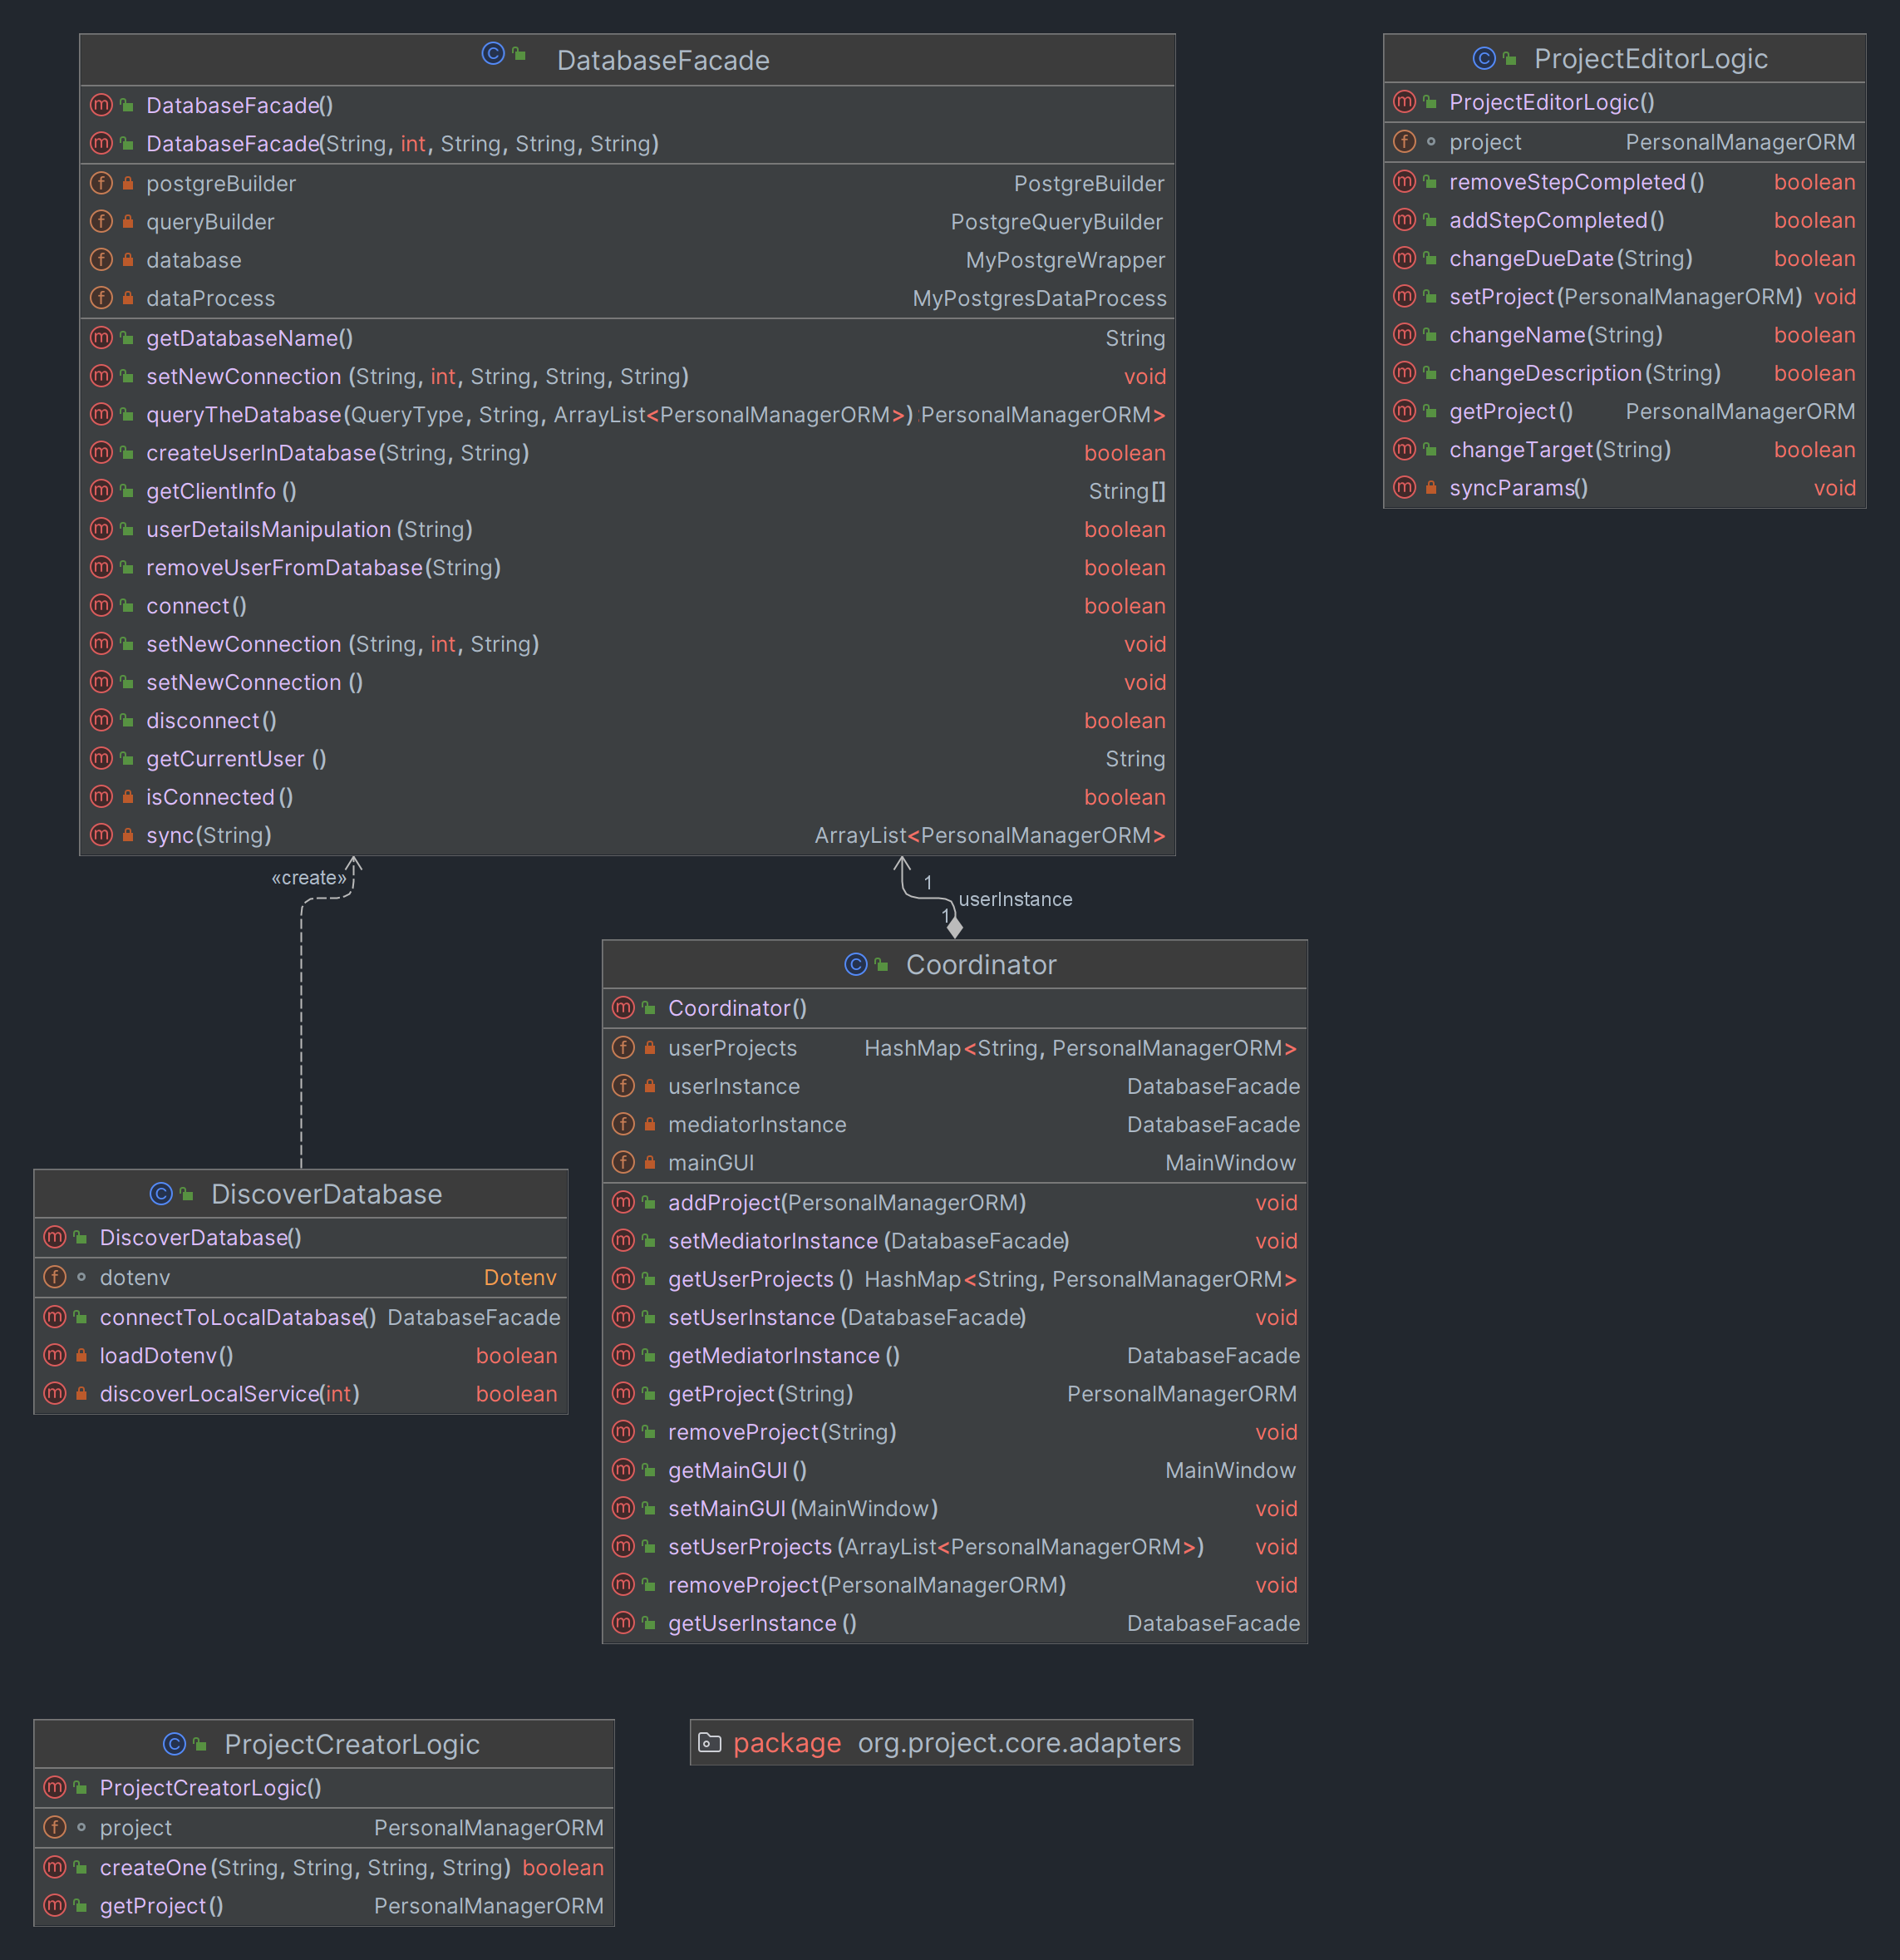
\includegraphics[width=0.8\textwidth]{Figures/UML/CORE}
        \caption{Diagramma delle classi del pacchetto org.project.core}
        \label{fig:diagrammaClassiCore}
    \end{figure}

    \subsection{org.project.database}\label{subsec:database}

    Il pacchetto org.project.database[\ref{fig:diagrammaClassiDatabase}] contiene le classi che
    implementano l'interazione con il database: connessione,
    creazione e modifica delle tabelle, inserimento, modifica e cancellazione dei dati tramite operazioni SQL/CRUD\@.
    Si tratta principalmente di classi wrapper per la libreria JDBC\@.

    \begin{figure}[tb]
        \centering
        \includegraphics[width=0.8\textwidth]{Figures/UML/DATABASE}
        \caption{Diagramma delle classi del pacchetto org.project.database}
        \label{fig:diagrammaClassiDatabase}
    \end{figure}

    \subsection{org.project.ORM}\label{subsec:ORM}

    Il pacchetto org.project.ORM[\ref{fig:diagrammaClassiORM}] contiene le classi che implementano l'object relational
    mapping, ovvero la mappatura tra le classi Java e le tabelle del database, ed i metodi per la gestione dei dati da
    essi contenuti.

    \begin{figure}[tb]
        \centering
        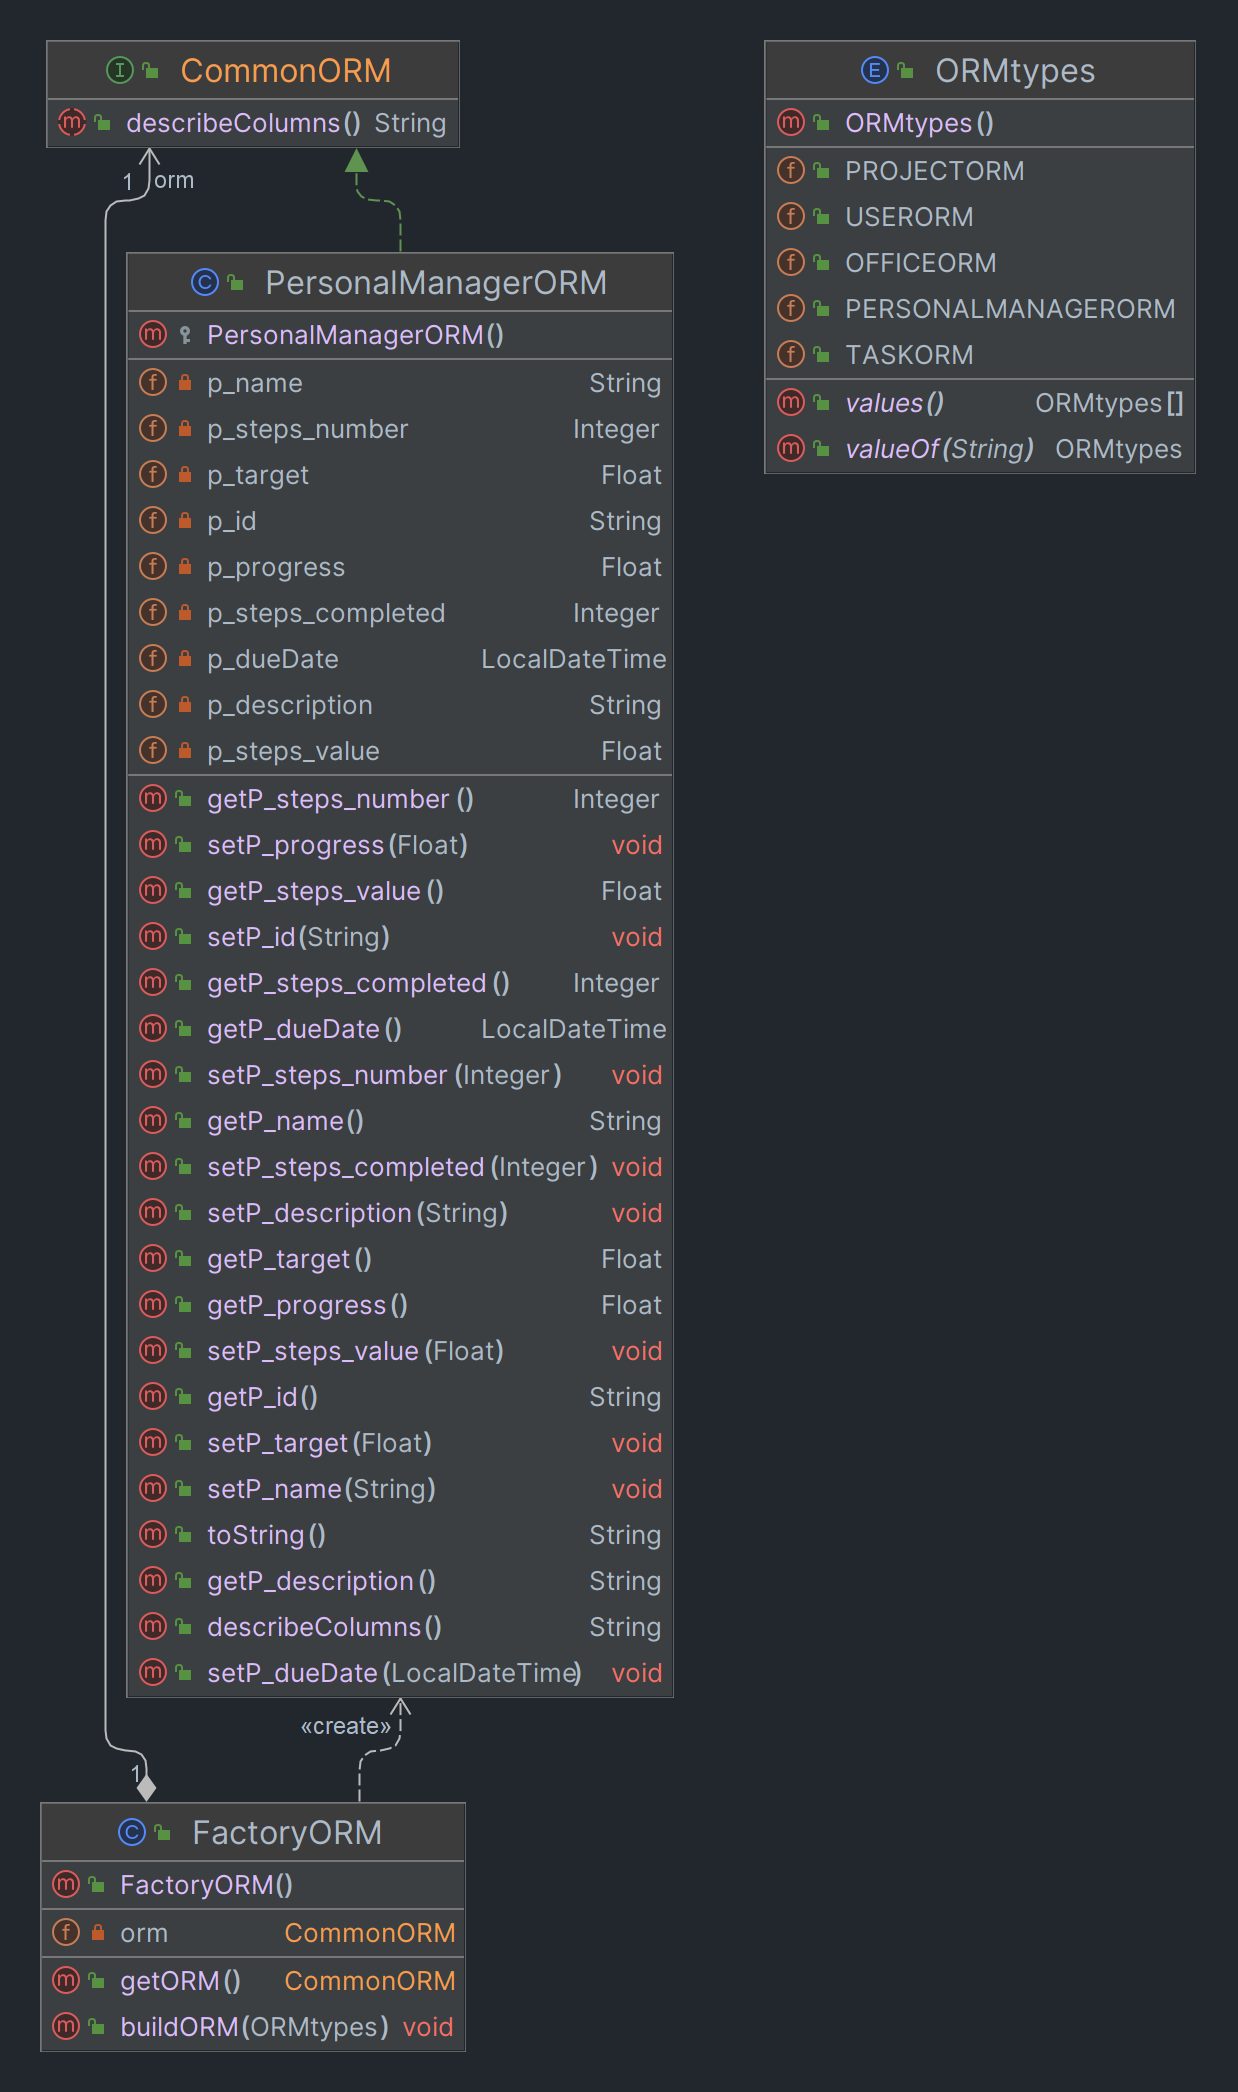
\includegraphics[width=0.8\textwidth]{Figures/UML/ORM}
        \caption{Diagramma delle classi del pacchetto org.project.ORM}
        \label{fig:diagrammaClassiORM}
    \end{figure}

    \subsection{org.project.GUI}\label{subsec:GUI}

    Il pacchetto org.project.GUI[\ref{fig:diagrammaClassiGUI}] contiene le classi che implementano la GUI del progetto.

    \begin{figure}[tb]
        \centering
        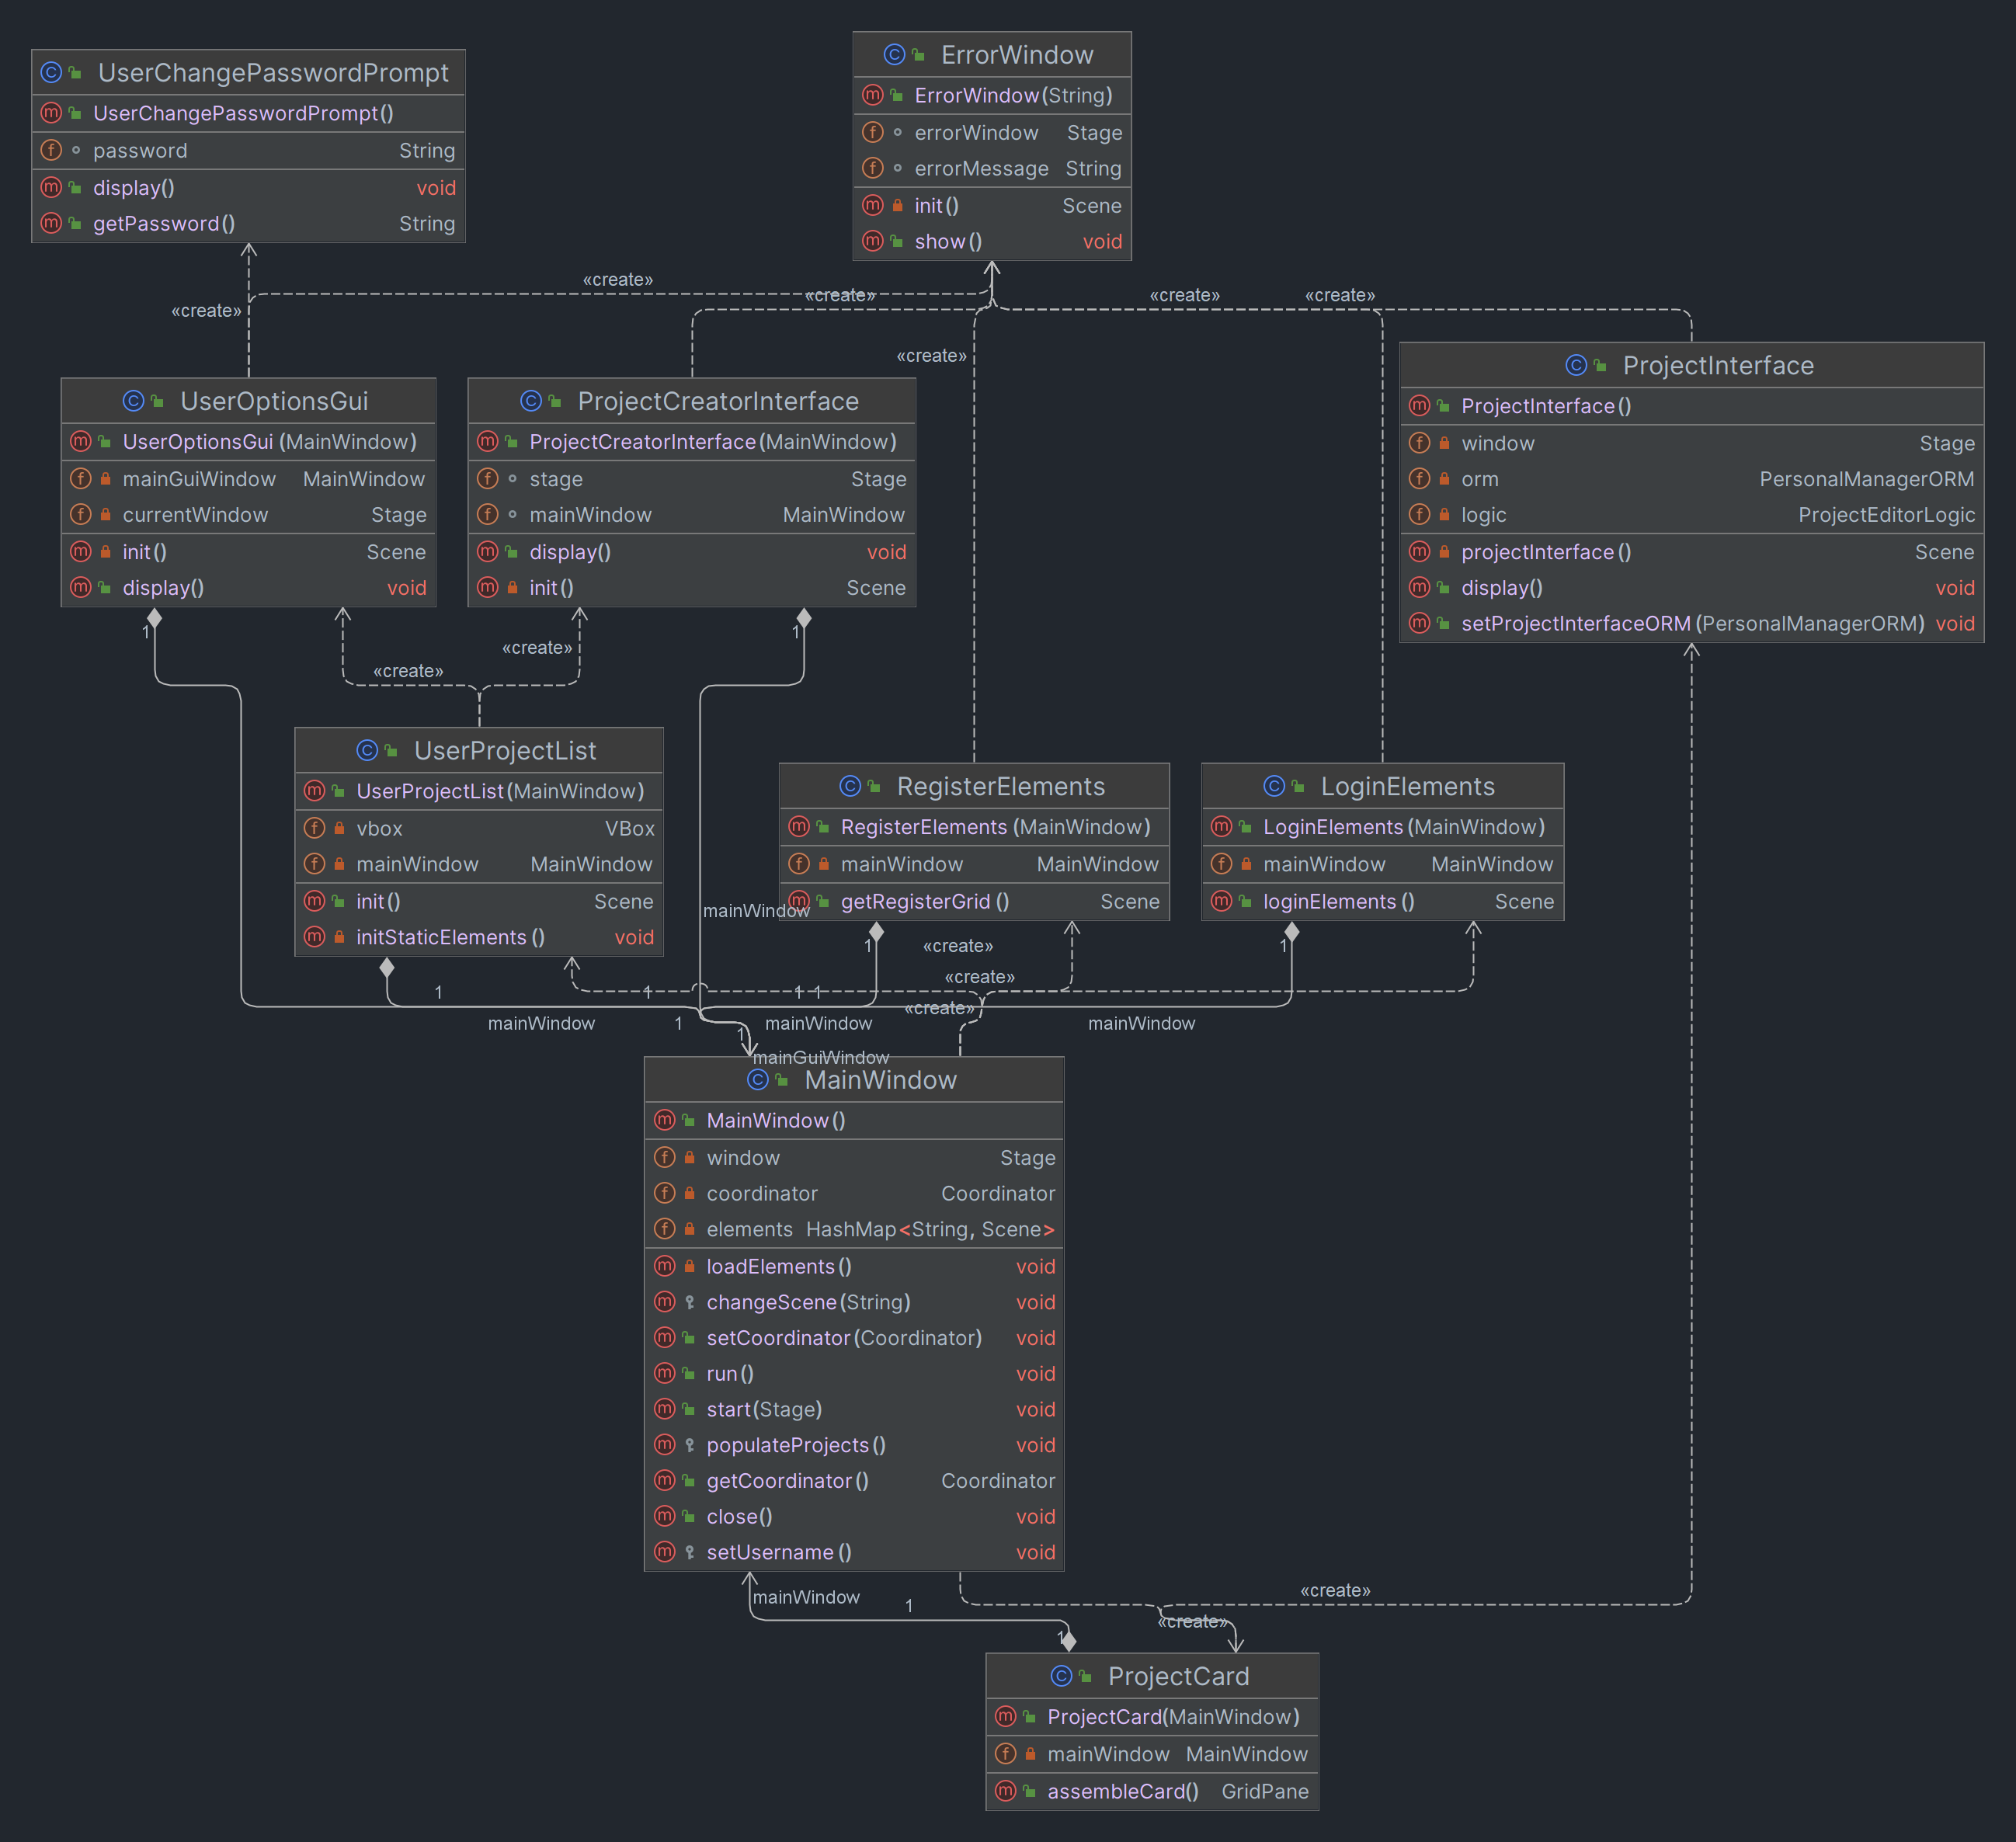
\includegraphics[width=0.8\textwidth]{Figures/UML/GUI}
        \caption{Diagramma delle classi del pacchetto org.project.GUI}
        \label{fig:diagrammaClassiGUI}
    \end{figure}

    \subsection{org.project.adapters}\label{subsec:adapters}

    Il pacchetto org.project.core.adapters[\ref{fig:diagrammaClassiAdapters}] contiene le classi che implementano
    l'adattamento dei dati tra le classi Java e il database, in particolare la conversione dei dati da e verso le
    classi Java e le tabelle del database.

    \begin{figure}[tb]
        \centering
        \includegraphics[width=0.8\textwidth]{Figures/UML/ADAPTERS}
        \caption{Diagramma delle classi del pacchetto org.project.core.adapters}
        \label{fig:diagrammaClassiAdapters}
    \end{figure}

%----------------------------------------------------------------------------------------
%	DETTAGLI IMPLEMENTAZIONE E CODICE
%----------------------------------------------------------------------------------------


    \section{Dettagli implementazione}\label{sec:dettagli}

    Questa sezione descrive i dettagli implementativi del progetto a livello di codice, e le scelte effettuate
    durante lo sviluppo a livello di architettura.

    \subsection{Architettura del progetto}\label{subsec:architettura}

    Il progetto è stato sviluppato utilizzando il paradigma di programmazione orientata agli oggetti, è stato
    fatto utilizzo di alcuni design pattern, ove è stato possibile si è cercato di aderire ai principi SOLID\@.
    L'intero progetto verte sull'esistenza di un database raggiungibile tramite composizione di un url a partire
    da dati pre\-esistenti, nel nostro caso un database PostgreSQL in localhost, che viene utilizzato come
    database di riferimento per la gestione dei dati e anche come autenticazione per l'accesso al programma.
    Il programma in se e per se può essere ridotto a un semplice client che si interfaccia con il database,
    ne manipola i dati e li visualizza in una GUI, questo è dovuto all'idea di partenza di ``imitare`` un webClient
    il cui scopo era interfacciarsi con un webApp nella rete.
    In alcune sue parti il programma è stato sviluppato in modo da essere facilmente estendibile,
    in particolare la parte relativa ai wrapper del database, altre parti come la GUI risultano più difficili(se
    non impossibili) da estendere o modificare.

    \subsection{Design pattern}\label{subsec:designPattern}

    Si è fatto uso di alcuni design pattern, nello specifico:

    \begin{itemize}
        \item \textbf{Builder}: implementato per la creazione dell'url del database e delle stringhe di query, con
        metodi in cascata, uno snippet del codice per la costruzione di query SQL è riportato in nella
        Lst.[~\ref{lst:snippetbuilder}].
        \item \textbf{Factory}: implementato per la creazione di oggetti di tipo ORM specifici per un dato tipo
        di tabella e database~\textsuperscript{\ref{lst:snippetfactory}}
        \item \textbf{Adapter}: implementato per la conversione dei dati tra le classi Java e le tabelle del
        database tramite oggetti creati tramite l'ORM factory, tramite l'interfaccia \textit{AdapterDataDB.java} vengono
        implementati dei metodi per la conversione dei dati nella classe concreta \textit{MyPostgresDataProcess.java}
        frammenti di codice delle due classi sono riportati nella Lst.[\ref{lst:snippetadapter}]

    \end{itemize}

    \begin{lstlisting}[caption={Frammento di codice da PostgreQueryBuilder.java}, label={lst:snippetbuilder}]
        ...

        /**
        * Builds the query depending on the query type
        *
        * @return the object with a built query set
        */
        public PostgreQueryBuilder buildQuery() {
            this.query = switch (this.type) {
            case INSERT -> addColumnsAndValues(insert);
            case UPDATE -> addColumnsAndValues(update);
            case DELETE -> addColumnsAndValues(delete);
            case SELECT -> select.replace("tablename", this.table);
            };
            return this;
        }

        public String getQuery() {
            return query;
        }
        ...
    \end{lstlisting}
    \newpage
    \lstinputlisting[caption={FactoryORM.java},label={lst:snippetfactory}]
    {../../src/main/java/org/project/ORM/FactoryORM.java}
    \lstinputlisting[caption={Interfaccia AdapterDataDB },label={lst:snippetadapter}]
    {../../src/main/java/org/project/core/adapters/AdapterDataDB.java}


\end{document}